\subsection{Overview}
The Phantom Head Desktop App is a hybrid signal processing platform designed to simulate, acquire, and visualize electrophysiological data. The software operates in two primary modes: \textit{Generated Mode} for synthesizing \gls{eeg}-like waveforms for phantom testing, and \textit{Measured Mode} for acquiring live biopotentials via OpenBCI hardware.

This manual outlines the interface architecture, operational procedures, and data management protocols.

\subsection{User Interface Architecture}

The user interface is divided into three primary functional zones.

\begin{figure}[h]
    \centering
    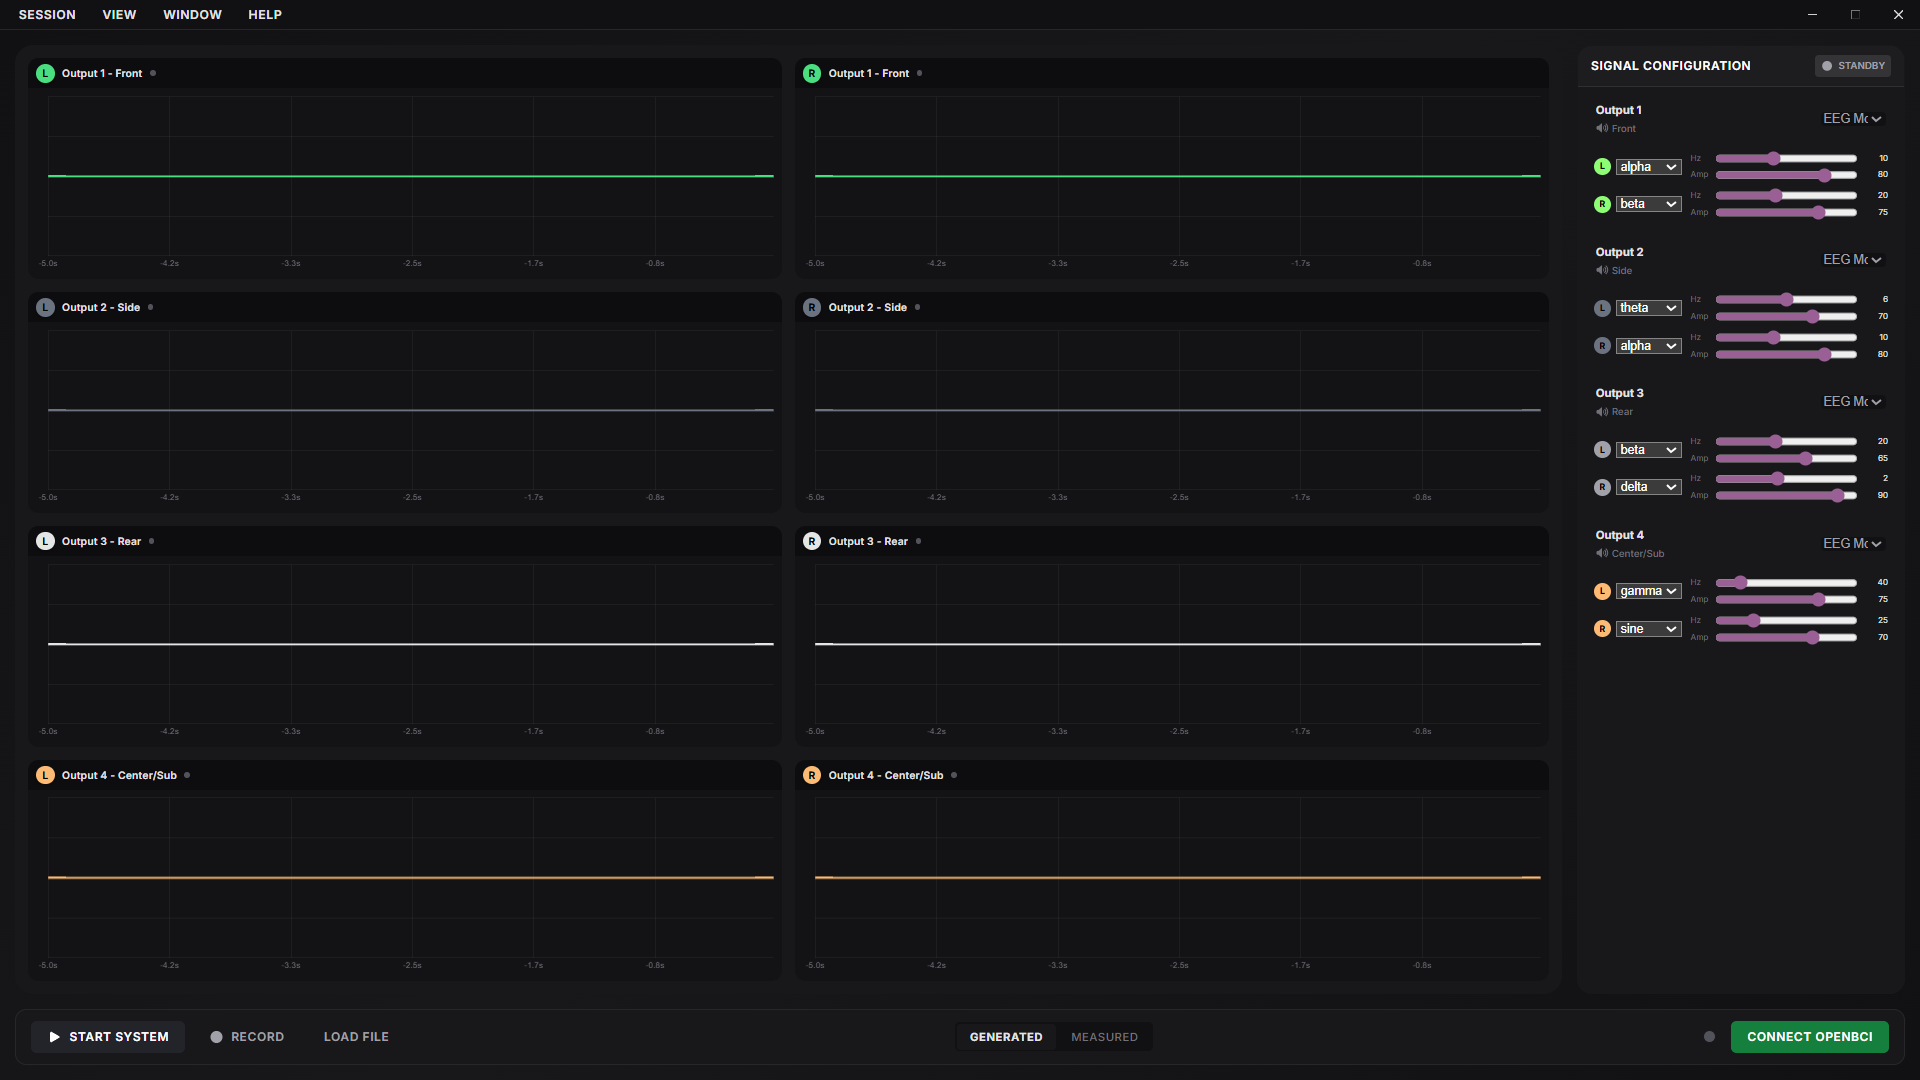
\includegraphics[width=\textwidth]{../../02_Images/gui_overview.png}
    \caption{Phantom Head Desktop App Main Interface}
    \label{fig:gui_overview}
\end{figure}

\subsubsection{Signal Visualization Area}
The central component of the interface is the real-time measurement display.
\begin{itemize}
    \item \textbf{Time Domain (X-axis):} Represents a rolling time window (default: 5 seconds).
    \item \textbf{Amplitude (Y-axis):} 
    \begin{itemize}
        \item In \textit{Generated Mode}: Normalized amplitude units (0{-}100\%).
        \item In \textit{Measured Mode}: Microvolts ($\mu V$).
    \end{itemize}
    \item \textbf{Channel encoding:} Each of the 8 channels is assigned a unique color for visual distinction. This color matches the corresponding sound output channel (based on the color code of the 7.1 sound card) or the channel of the OpenBCI Cyton board.
\end{itemize}

\subsubsection{Output Control Modules}
The system utilizes four distinct output modules, each controlling a stereo pair of channels (left/right), totaling 8 channels.
\begin{itemize}
    \item \textbf{Output 1:} Front left and right outputs of the 7.1 sound card.
    \item \textbf{Output 2:} Side left and right outputs of the 7.1 sound card.
    \item \textbf{Output 3:} Rear left and right outputs of the 7.1 sound card.
    \item \textbf{Output 4:} Center and subwoofer outputs of the 7.1 sound card.
\end{itemize}

\subsubsection{Global Control Bar}
Located at the bottom of the window, this toolbar contains signal generation controls (Play, Stop, Record), mode selection, and hardware connection interfaces.

\subsection{Operating Modes}

The software functions in two mutually exclusive modes, toggled via the \textit{View} selector.

\subsubsection{Generation Mode (Simulation)}
This mode synthesizes artificial \gls{eeg} signals for hardware verification and educational demonstration. It allows for the independent manipulation of frequency, amplitude, and waveform topology for all 8 channels.
\begin{itemize}
    \item \textbf{Waveform Selection:} Select the desired topology (e.g., Alpha) from the module dropdown. The system automatically snaps the frequency range to the standard \gls{eeg} band that corresponds to the selected waveform.
    \item \textbf{Amplitude Modulation:} Adjust the signal strength (0{-}100) to control the voltage output to the phantom head via the volume of the audio soundcard.
    \item \textbf{Audio Feedback:} Real-time sound of signals is provided via stereo output (Left/Right channel mixing).
    \item \textbf{Import option:} Import an EDF file and select a channel from the dropdown menu to generate it.
\end{itemize}

\begin{figure}[H]
    \centering
    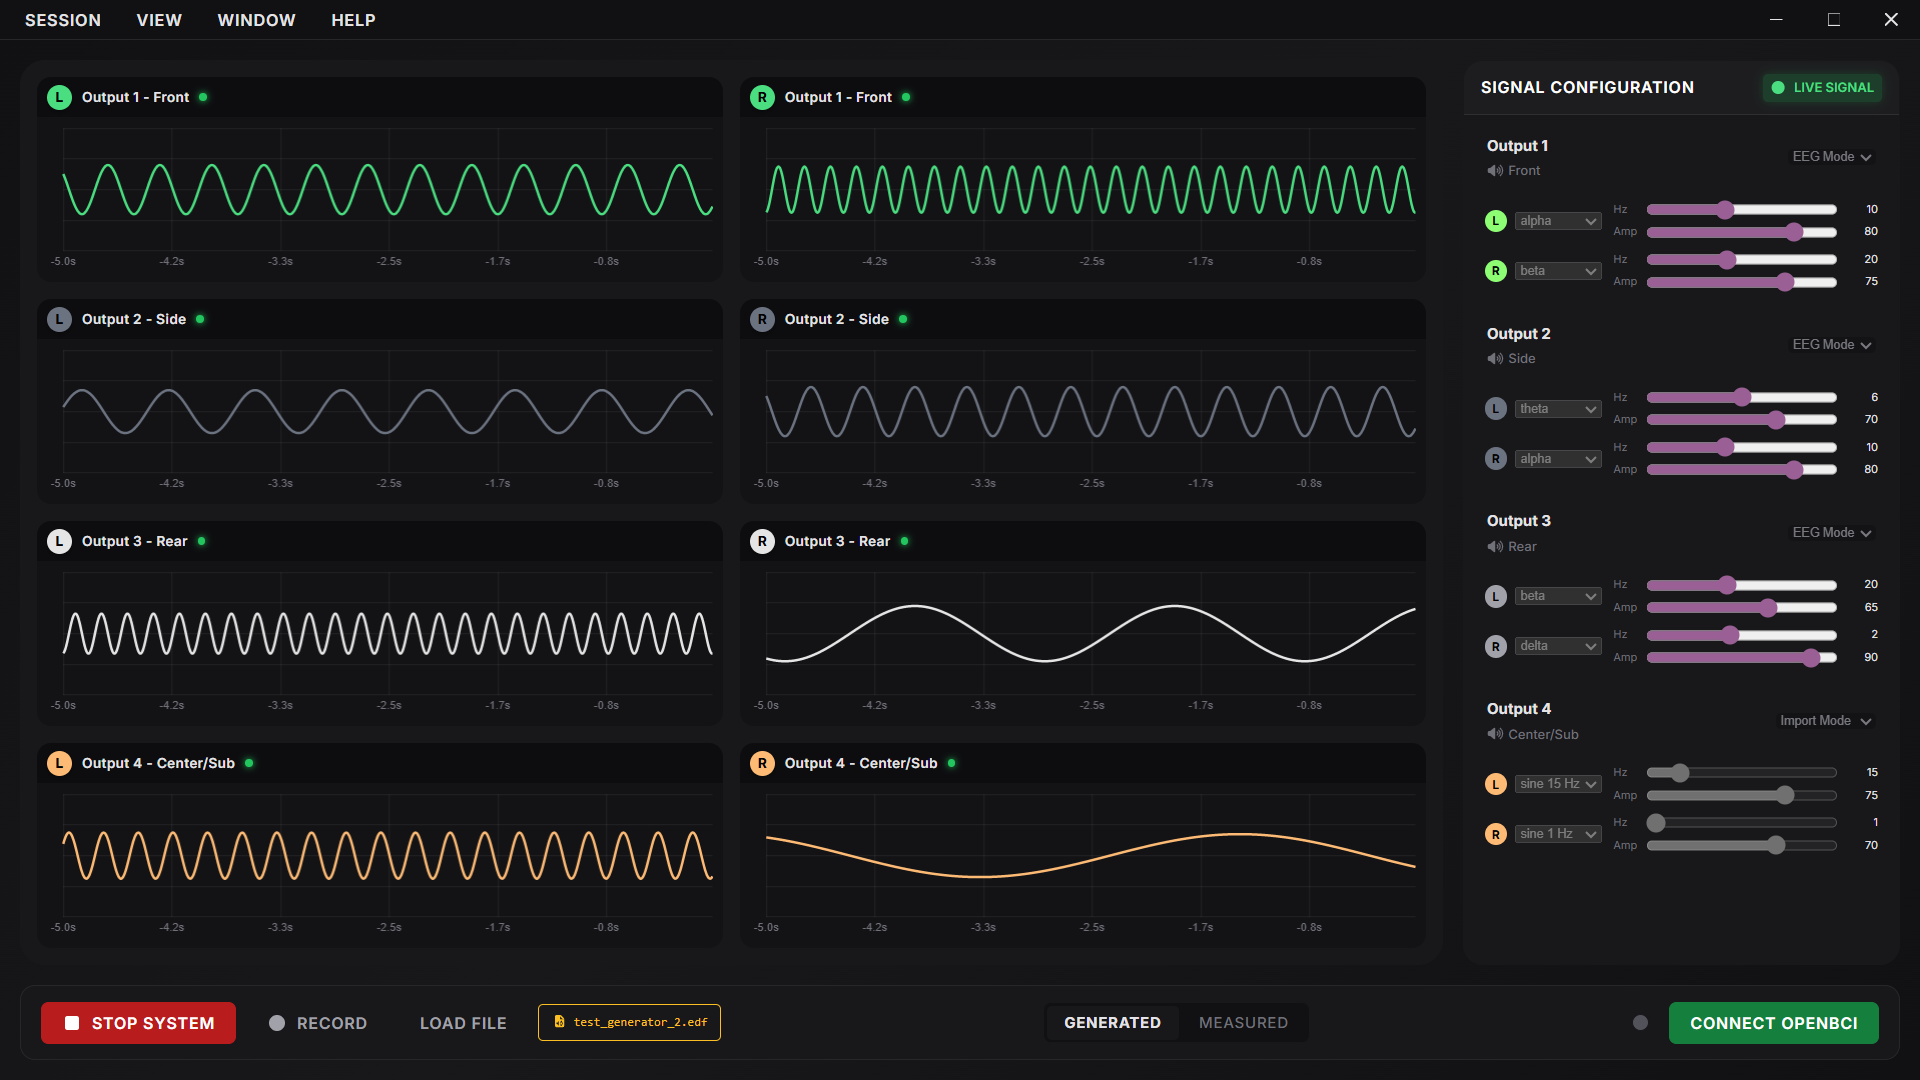
\includegraphics[width=\textwidth]{../../02_Images/generated_mode.png}
    \caption[Generation mode interface]{Generation mode interface, with file uploaded in EDF format}
    \label{fig:generated_mode}
\end{figure}

\subsubsection{Measuring Mode (Acquisition)}
This mode interfaces directly with the OpenBCI Cyton biosensing board.
\begin{itemize}
    \item \textbf{Sampling Rate:} 250 Hz (Hardware native).
    \item \textbf{Signal Conditioning:} Raw data undergoes automatic DC offset removal and bandpass filtering prior to visualization.
    \item \textbf{Dynamic Range:} up to $\pm 1000 \mu V$, with time window adjustment from 1 to 10 seconds.
\end{itemize}

\begin{figure}[H]
    \centering
    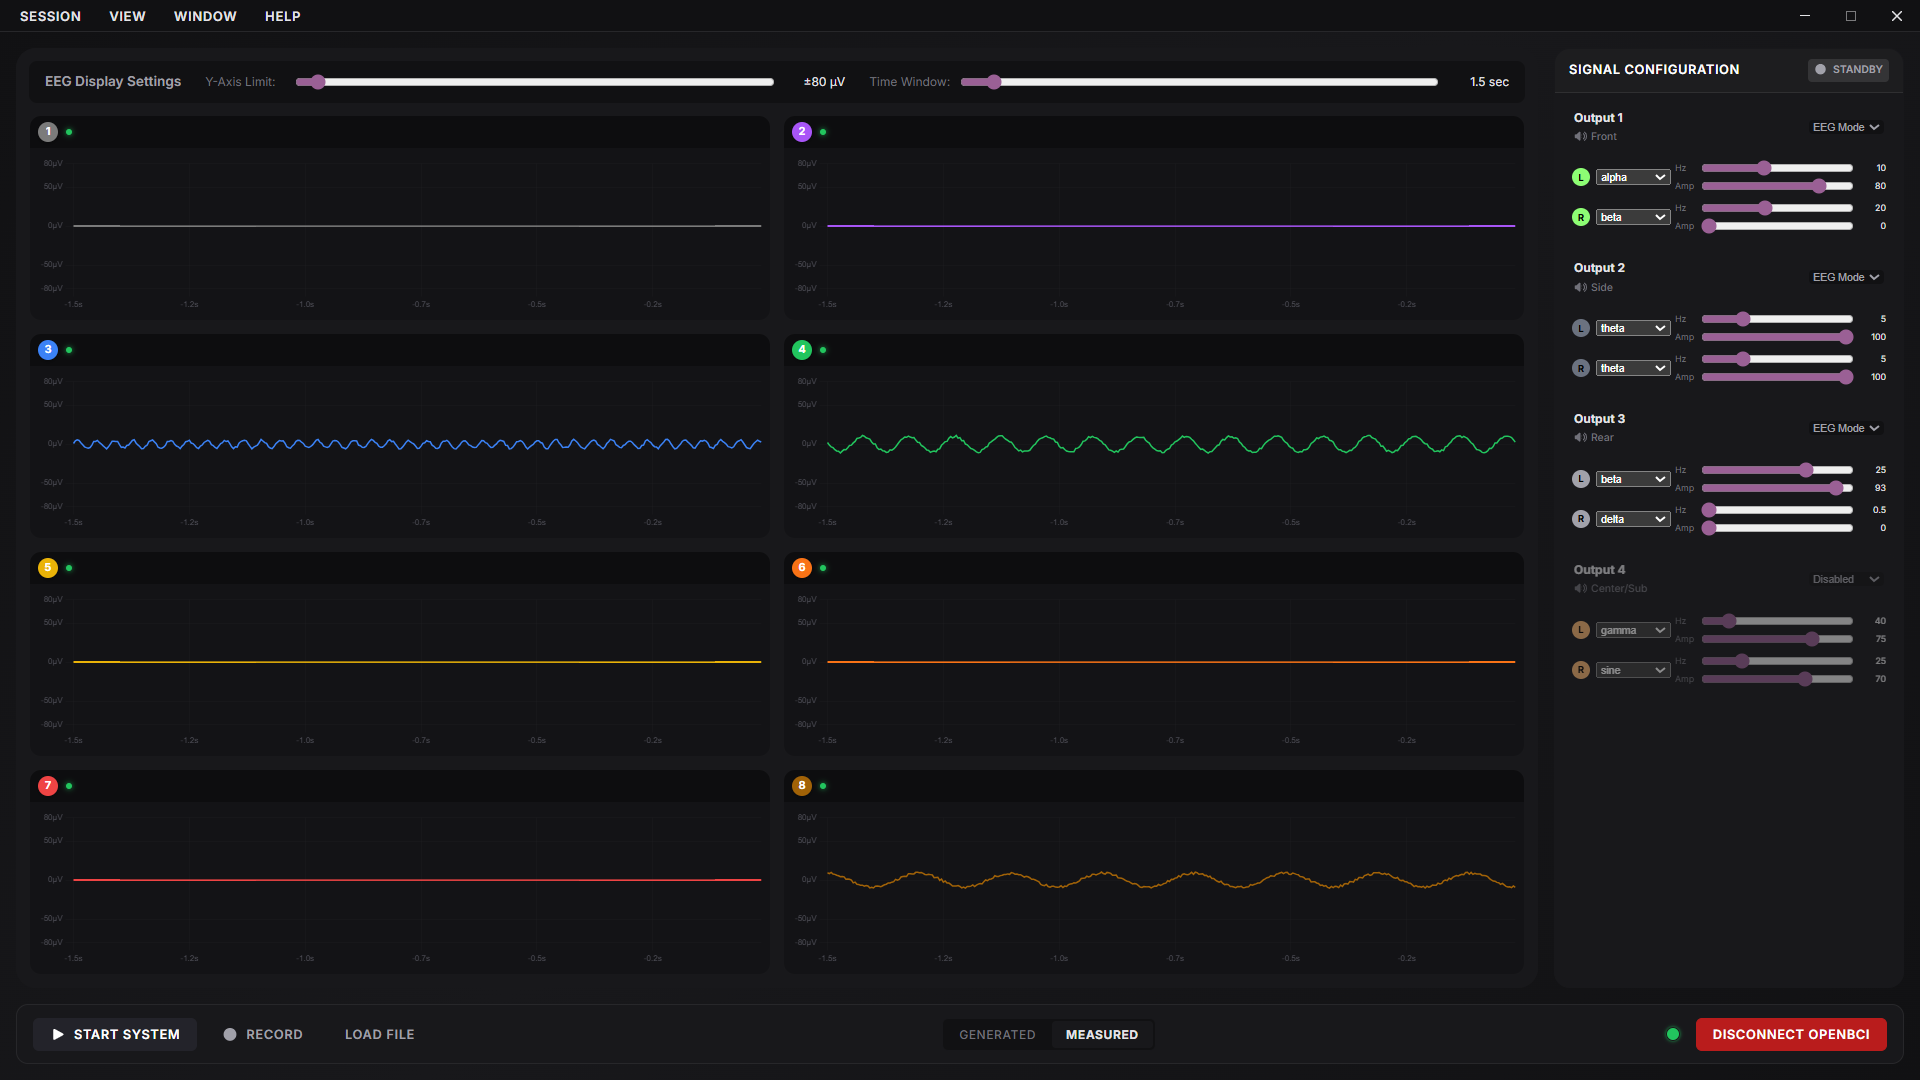
\includegraphics[width=\textwidth]{../../02_Images/measured_mode.png}
    \caption{Measuring mode interface}
    \label{fig:measured_mode}
\end{figure}

\subsubsection{Application Menus}

The application includes standard menu options for session management, viewing configurations (zoom, fullscreen, reload), window controls, and help resources.

\begin{figure}[H]
    \centering
    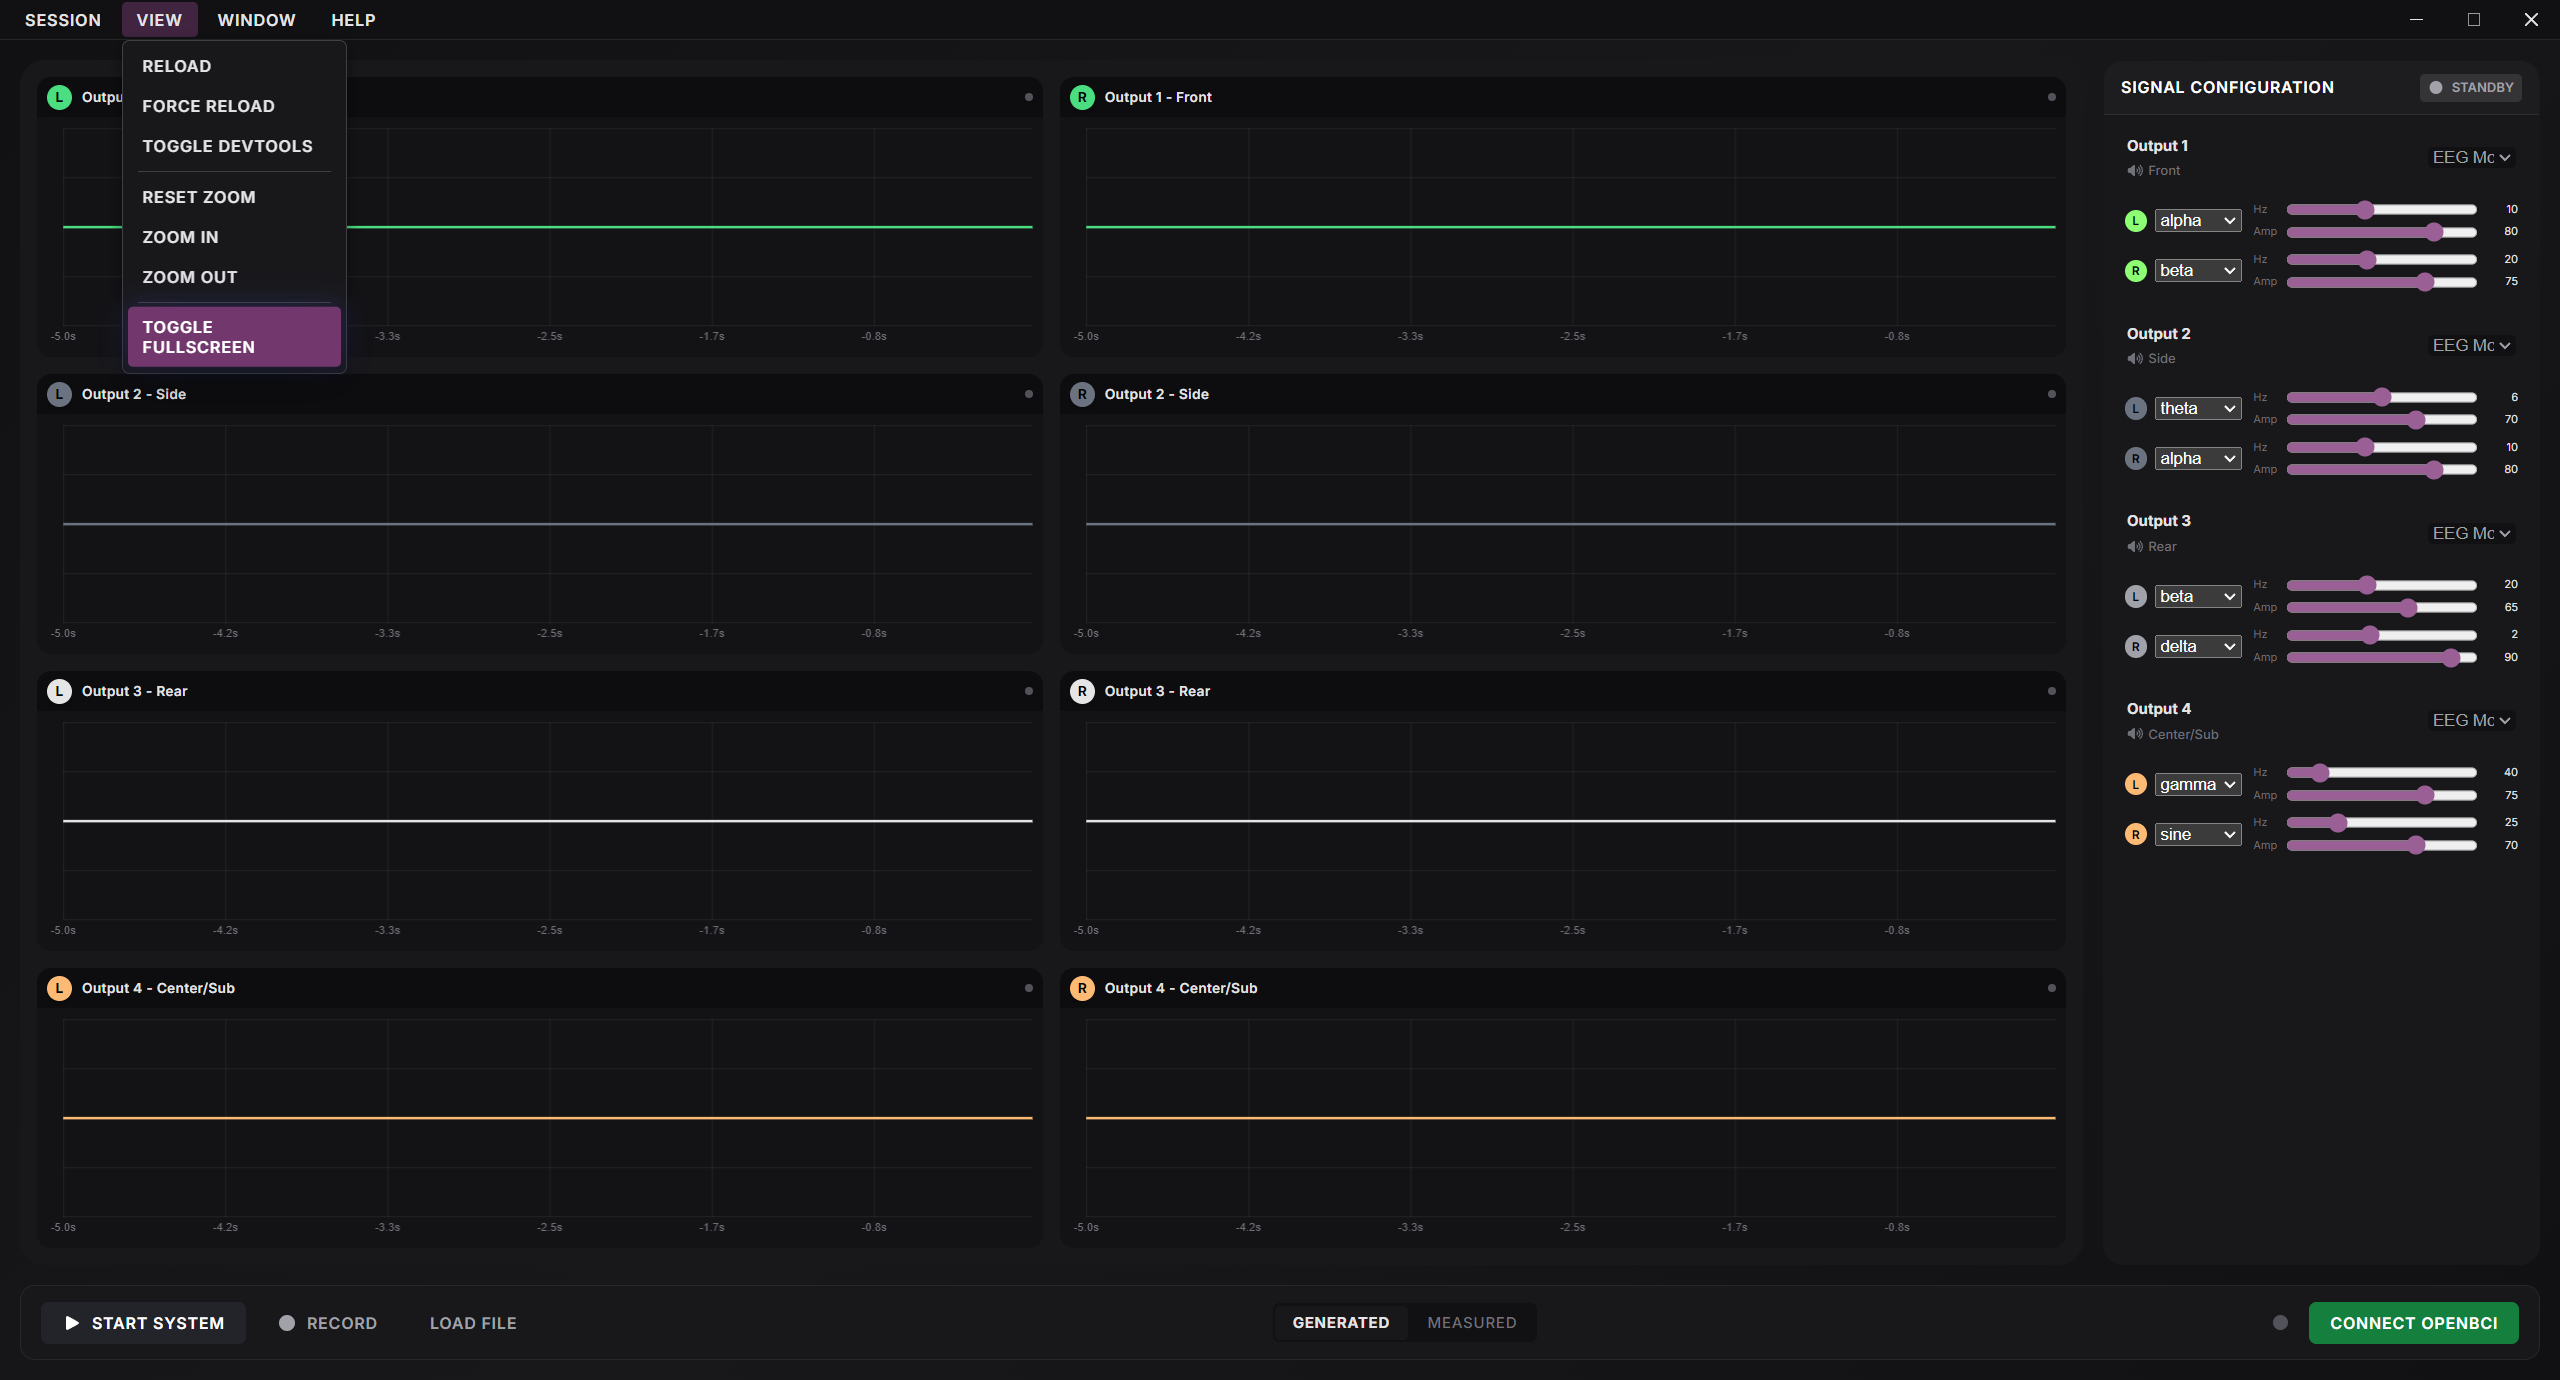
\includegraphics[width=\textwidth]{../../02_Images/view_menu.png}
    \caption{View menu}
    \label{fig:view_menu}
\end{figure}

\begin{figure}[H]
    \centering
    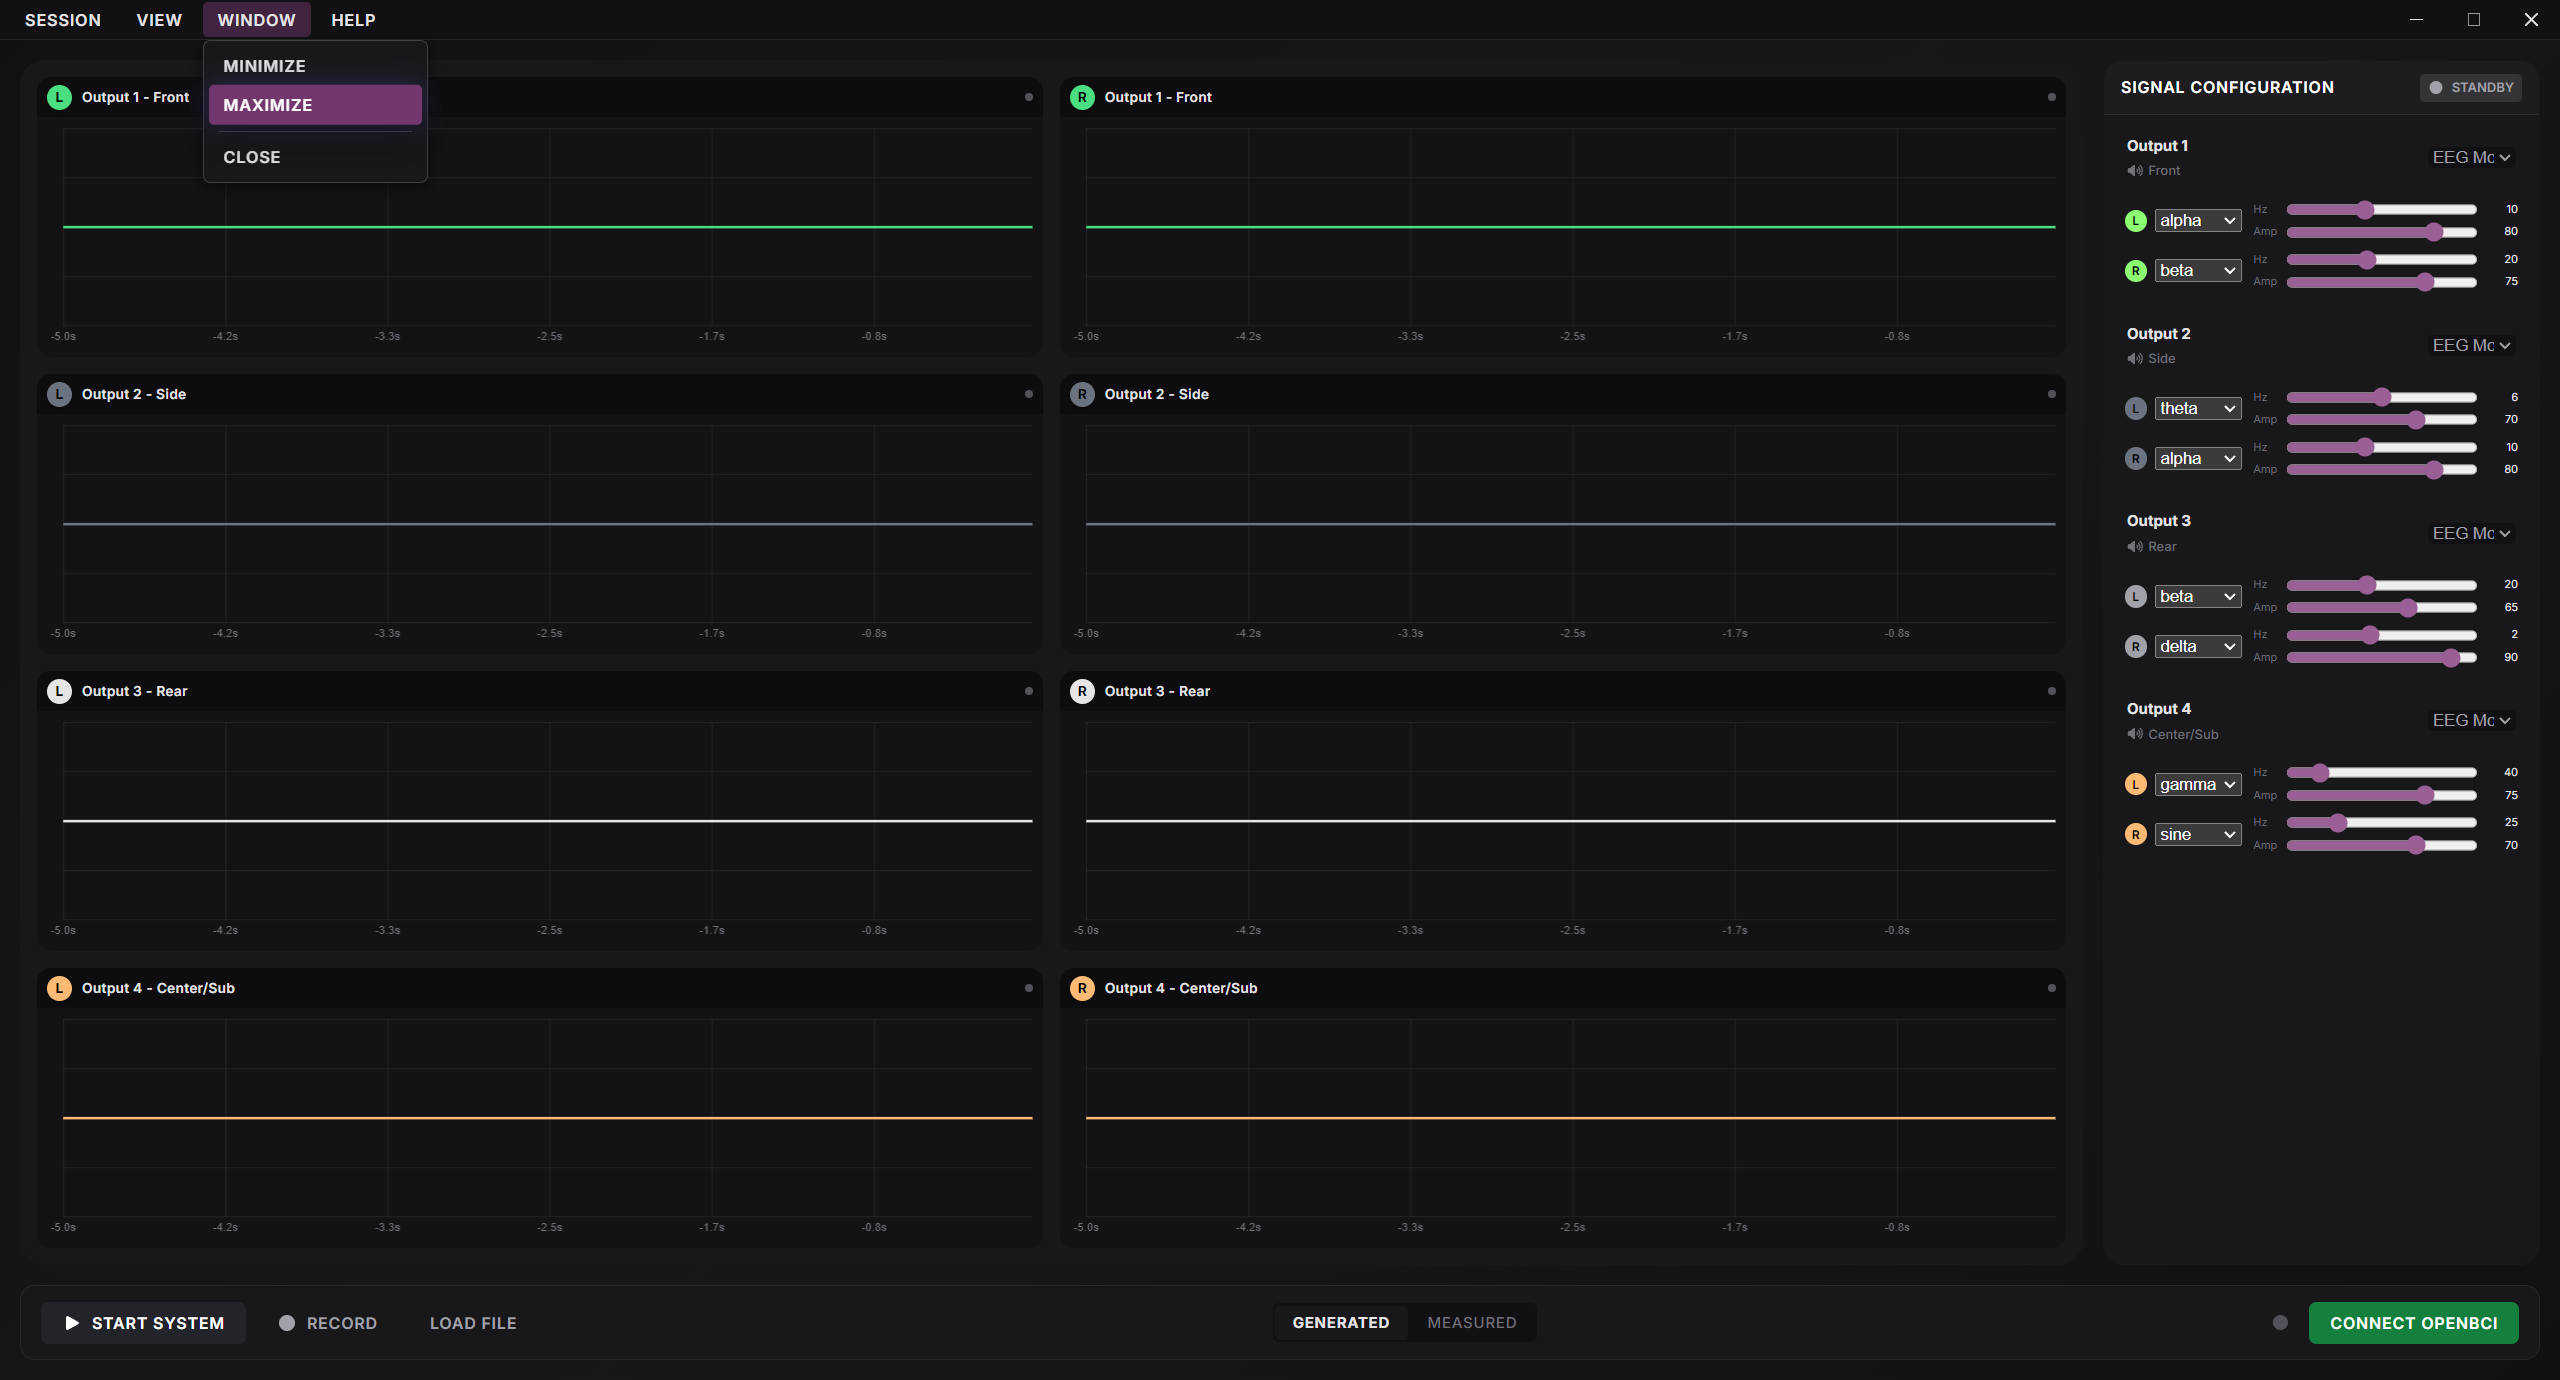
\includegraphics[width=\textwidth]{../../02_Images/window_menu.png}
    \caption{Window menu}
    \label{fig:window_menu}
\end{figure}

\begin{figure}[H]
    \centering
    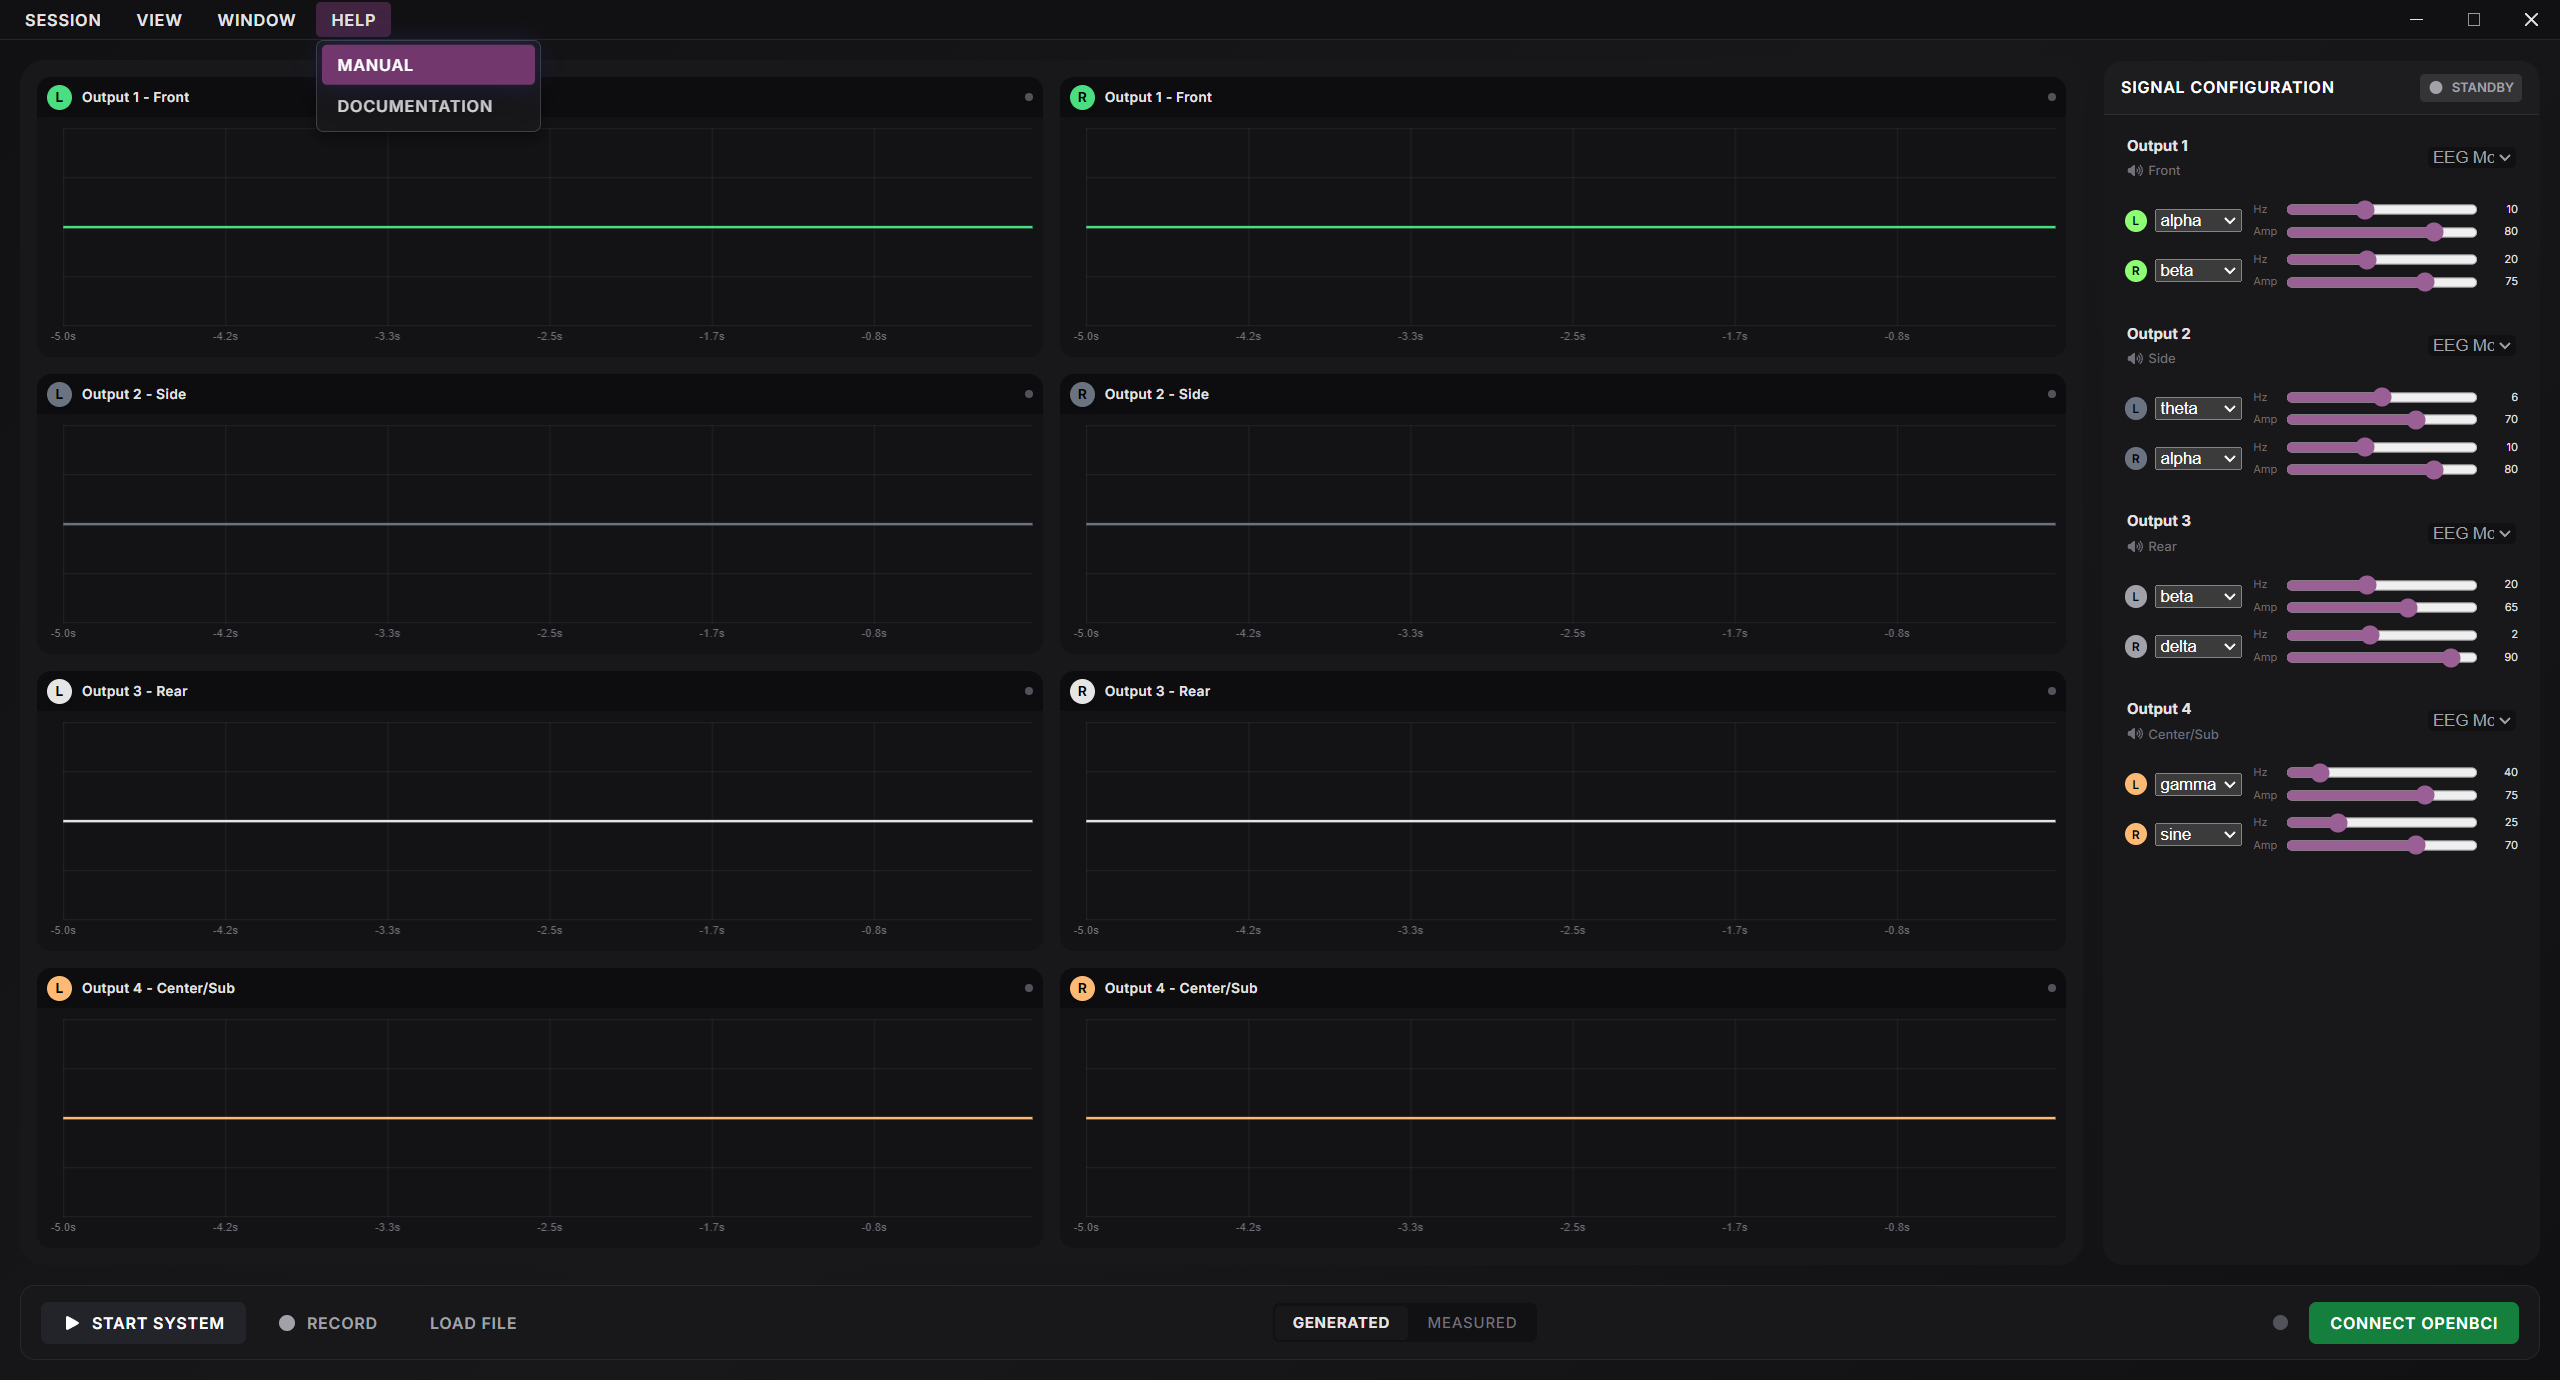
\includegraphics[width=\textwidth]{../../02_Images/help_menu.png}
    \caption{Help menu}
    \label{fig:help_menu}
\end{figure}

\subsection{Hardware Integration (OpenBCI)}

\subsubsection{Connection Procedure}
To initialize a hardware session with the OpenBCI Cyton board:
\begin{enumerate}
    \item Ensure the USB dongle is connected and the board is powered on.
    \item Click the \textbf{Connect OpenBCI} button in the Global Control Bar.
    \item The status indicator provides visual feedback:
    \begin{itemize}
        \item \textbf{Gray:} Disconnected / Idle.
        \item \textbf{Pulsing:} Handshaking / Connecting.
        \item \textbf{Green:} Connection established; data stream active.
    \end{itemize}
    \item Switch the View Mode to \textbf{Measured} to visualize the incoming data stream.
\end{enumerate}

\subsection{Data Acquisition and Export}

The Phantom Head Desktop App includes a logging engine capable of recording session data in multiple formats.

\subsubsection{Recording a Session}
Clicking the \textbf{Record} button initiates the logging buffer. The system captures:
\begin{itemize}
    \item Raw time-series data for all 8 channels.
    \item High-precision timestamps.
    \item Event markers (parameter changes, mode switches).
\end{itemize}

\subsubsection{Export Formats}
Upon concluding a recording, the user obtains a ZIP archive containing:

\paragraph*{JSON (JavaScript Object Notation)}
Archival and replay. It preserves metadata, event logs, and full-resolution data.

\paragraph*{CSV (Comma-Separated Values)}
Suitable for statistical analysis in external software (e.g., MATLAB, Python, Excel).

\paragraph*{WAV (Audio)}
Exports the generated signal as a standard 16-bit PCM audio file.~\textit{Note: Only available for generated signals.}